\documentclass[a4paper,12pt]{report}
\usepackage{geometry}
 \geometry{
 a4paper,
 total={210mm,297mm},
 left=25mm,
 right=25mm,
 bottom=25mm,
 top=25mm,
 }
\usepackage[english]{babel}
\usepackage[T1]{fontenc}
\usepackage[utf8]{inputenc}
\usepackage{lmodern}
\usepackage{microtype}
\usepackage{graphicx}
\usepackage{caption} 
\usepackage{titling}
\usepackage[colorlinks=true,linkcolor=black,urlcolor=blue]{hyperref}
\usepackage{indentfirst}
\usepackage{siunitx}
\usepackage{amsmath}
\usepackage{multicol}
\usepackage[backend=biber,style=ieee]{biblatex}
\nocite{*}
\addbibresource{Biblio.bib}



\title{Bibliographical Project \\ [1ex]\large X-Rays and Radiography \\ (based on the work of Wilhem Röntgen)  }
\author{}

\date{October 1, 2023} 

\begin{document}

\begin{titlepage}
  \centering
  \vspace{3cm}
  \Huge{\textbf{Bibliographical Project}}\\
  \vspace{1cm}
  \Large{X-Rays and Radiography \\ (based on the work of Wilhem Röntgen)} \\
  \vspace{0.5cm}
  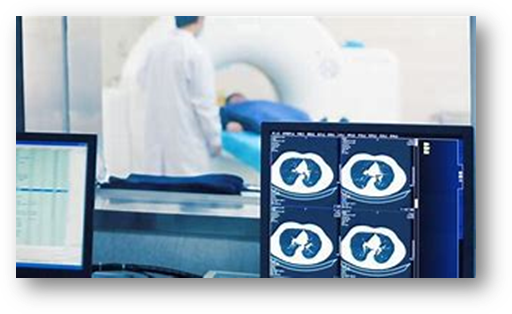
\includegraphics[scale=1]{xray.png}\\
  \vspace{0.5cm}
  \\
  \vspace{1.5cm}
  \large{\textit {Under the supervision of A.LEHMANN and F.MANDIJA}} \\
  \vspace{1.5cm}
  \thedate \\
  \vspace{2cm}
  
\includegraphics[scale=0.6]{Isep.jpg}\\
  
\end{titlepage}





\begin{abstract}
  W.C Röntgen's work was revolutionary. X-rays are father of radioactivity and great-father of quantum mechanics. We try here to produce a synthesis of X-ray discovery by the physician. In a historical and practical context. Also we introduce pionneers application of this new-kind of radiation now well-known.
\end{abstract}
\tableofcontents
\addcontentsline{toc}{section}{Introduction}


\setlength{\parskip}{10pt}


\newpage
\begin{flushright}
  \textit{In the fields of observation, chance favors only the prepared mind. Louis Pasteur, 1854}
\end{flushright}
\section*{Introduction}

Before starting explanation of Wilhelm Röntgen's work and discovery we have made the choice to introduce a brief abstract on current theorical aspect of X-rays. There are several elementary points usefull to understand. Please keep in mind during lecture those notions.


\subsection*{Basics of X-rays's physics}
X-rays, also recognized as X-radiation, are a form of electromagnetic radiation characterized by
high energies. Radiation categorization is based on its wavelength \(\lambda\), representing the length of
one complete wave cycle. This wavelength can alternatively be defined in terms of frequency \(\nu\)
and the propagation speed of the wave, denoted as the speed of light. The relationship
between these parameters is fundamental in characterizing different types of radiation, illustrating
the interplay between wavelength, frequency, and the speed of light in the electromagnetic
spectrum.

\begin{equation}
  \lambda = \frac{c}{\nu}
\end{equation}


The energy of a photon is characterised by the following formula :
\begin{equation}
E= \frac{hc}{\lambda}= h\nu\ = [eV]
\end{equation}


The energy of photons can be expressed using Planck's constant \(h \approx 6.626.10^{-3} J.s\) and the
speed of light \(c \approx 2.997.10^8 m.s^{-1}\). This energy is directly connected to the wavelength \(\lambda\) or
frequency \(\nu\) of the photon, measured in electron volts [eV]. The relationship reveals that the
photon energy is directly proportional to its frequency and inversely proportional to its
wavelength. In simpler terms, an increase in frequency corresponds to higher energy, highlighting
the direct relationship between these fundamental properties of photons.

These high-energy photons possess short wavelengths, resulting in exceptionally high
frequencies. The pivotal parameter defining all photons is their radiation frequency, which, in
turn, determines their energy. Photons are classified based on their energies, spanning from low-
energy radio waves and infrared radiation, progressing through visible light, and culminating in
high-energy X-rays and gamma rays.
\newpage

Here is the complete electromagnetic spectrum :
\begin{center}
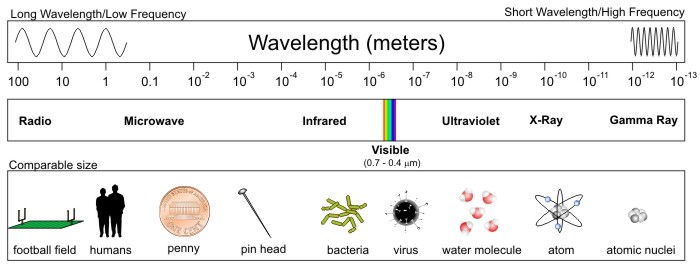
\includegraphics[scale = 2.4]{elecSpec.jpg}
\captionof{figure}{The Electromagnetic Spectrum (Credit : David Babb, PennState)}

\label{elecSpec}
\end{center}

It is relevant to note that \textit{X-rays and Gamma-rays} are also called \textit{ionizing radiation} meaning they have engough energy to transform atom they go through into ions. Hence, the atom loose or receive an electron. This can make matter unstable.

\subsection*{Bremsstrahlung effect or braking radiation}

In today's world, X-rays are generated using specialized X-ray machines. These machines offer
the flexibility to adjust both current and voltage settings, enabling the manipulation of the
properties of the X-ray beam produced. This capability allows for the application of distinct X-
ray beam spectra tailored to specific body parts during medical imaging procedures.

Nowadays, Science explains the generation of X-rays  the \textit{Bremsstrahlung }effect from the German, braking radiation. 
According to the following Maxwell-Lorentz equations, "any electric charge with a variating speed emits an electromagnetic radiation".\footfullcite{BibnumDécouverteX}

Maxwell's equations:
\begin{align}
  \nabla \cdot \vec{E} &= \dfrac{\rho}{\varepsilon_0} \\
  \nabla \cdot \vec{B} &= 0 \\
  \nabla \times \vec{E} &= -\dfrac{\partial \vec{B}}{\partial t} \\
  \nabla \times \vec{B} &= \mu_0 \vec{J} + \mu_0 \varepsilon_0 \dfrac{\partial \vec{E}}{\partial t}
\end{align}

Lorentz force equation:
\begin{equation}
  \vec{F} = q(\vec{E} + \vec{v} \times \vec{B})
\end{equation}

You can observe on Figure \ref{brakingEff}  that emitted electrons are deviated by the positive charge of target's atoms.  

\begin{center}
  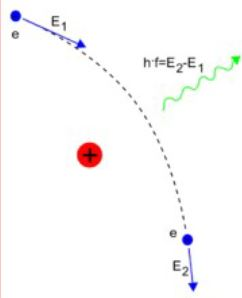
\includegraphics[scale = 1.5]{brakingEff.jpg}
  \captionof{figure}{\textit{Bremsstrahlung effect} }
  \label{brakingEff}
\end{center}

During the deviation, a photon is emitted by the atom. This is the radiation. The energy balance of the interaction is given by : 

\begin{equation}
  E'_c - E_c = h\nu\
\end{equation}

The majority of X-rays exhibit wavelengths that fall within the range of 0.01 to 10 nanometers (corresponding to frequencies of \(3.10^{16} Hz\) to \(3.10^{19} Hz\) ), with energies spanning from 100
eV to 100 keV. Notably, X-ray wavelengths are shorter than those of ultraviolet (UV) rays and
generally longer than those of gamma rays.







\chapter{Historical Background}
\section{Radiation Understanding in the Late 19\textsuperscript{th} century}
The 19th century stood as an era dominated by an abundance of brilliant minds, particularly in
the field of physics, showcasing an unprecedented concentration of intellectual prowess in the
department of sciences. This period unfolded with a cascade of remarkable discoveries,
groundbreaking inventions, precise measurements, and novel theories.

It was characterized by significant advancements in different domains in physics like electricity
and thermodynamics, leading to transformative technical and medical applications. These
innovations collectively revolutionized our world, shaping the course of history and influencing
the present day.

In the late 19th century, significant progress was made in the exploration of atomic structure and
radiation. We could for example talk about Dmitri Mendeleev groundbreaking contribution in
1869 with the introduction of the periodic system of elements. Going back in time, William
Herschel's 1800 discovery of infrared rays using a prism revealed previously unseen rays beyond
the red spectrum, termed "calorific rays.". Johann Wilhelm Ritter, in 1801, explored ultraviolet
radiation, noting its darkening effect on silver chloride. James Clerk Maxwell's equations laid
theoretical groundwork, proposing that visible light, infrared, and ultraviolet rays are
disturbances in the electromagnetic field. Heinrich Hertz's 1887 deliberate creation of radio
waves applied Maxwell's equations practically. 

W.C. Röntgen was especially interested in the work of Mrs. Hertz and Lenard,two german researchers. Their worked on cathod-rays, and the electricity discharges in low-pressure gazes. Röntgen studies on this subject is fundamental for his future discovery. 
\chapter{Life and Career of Wilhelm Conrad Röntgen}
\section{Early Life of an enthusiastic genius}

\begin{center}
  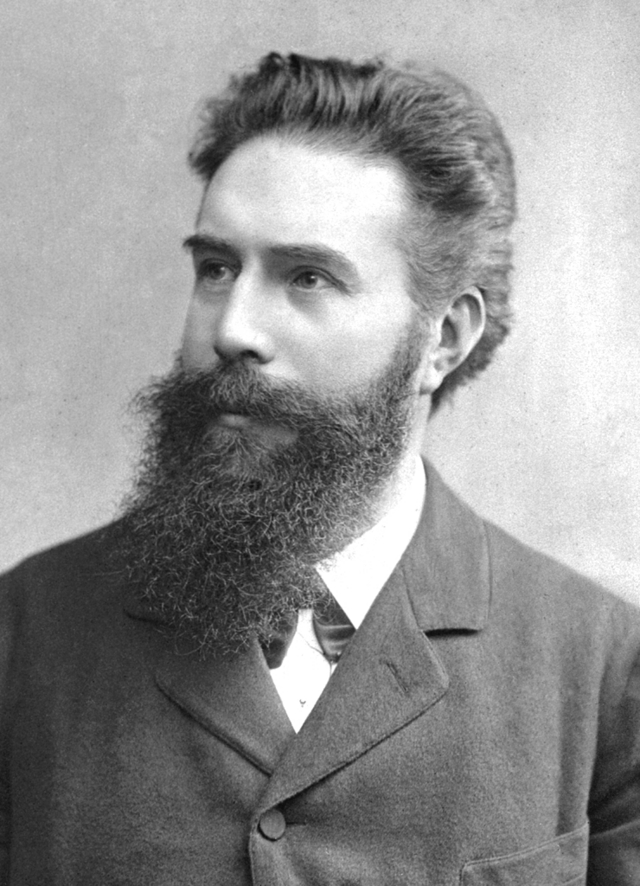
\includegraphics[scale=0.3]{roentgen.png}
  \captionof{figure}{WIlhelm Conrad Röntgen}
  \label{fig=Röntgen}
\end{center}

Sometimes history is made of incredible destiny. Wilhelm Conrad Röntgen, born on March
27th, 1845 near Dusseldorf, Germany was not incline to brillant physics studies. His father a
sheet merchant did not push him throughout this way. Röntgen's early life was marked by a
move to Netherlands for his father's business. Röentgen's journey into science began at the
Utrecht Technical School at the age of 16, leading to a diploma in engineering three years later.
His academic pursuits continued, culminating in a Ph.D. under the guidance of A.E.E. Kundt,
focusing on gas properties.

Röentgen was described as a tall, dark, and slender man, maintained a modest and meticulous
approach to his scientific endeavors. Röentgen's career progressed with his mentor, Kundt, to the
University of Würzburg and later to Strasbourg, where he became an associate professor in
theoretical physics. In 1879, he assumed the position of professor of physics at Giessen,
eventually returning to Würzburg in 1888. It was here, on November 8, 1895, that Röentgen
accidentally observed what he later named X-rays. Promptly sharing his findings with the
Physics-Medical Society of Würzburg in December, his discovery quickly captivated the global
scientific community.

The Vienna Presse reported the phenomenon in January 1896, highlighting the potential
applications of X-rays in medicine. The discovery opened doors to radiology, with practical uses
imaging, such as locating bullets in the human body and visualizing fractures before surgery.
Despite initial challenges in applying X-rays to obstetric \footfullcite{perinatal} and prenatal diagnosis due to limited
penetration through tissues, subsequent decades saw significant progress, particularly in the
1930s with the development of more powerful X-ray beams.

\section{Röntgen's groundbreaking experiment}

On November 8, 1895, Röntgen covered a Crookes tube with black cardboard. The Crookes tube
was powered by a Ruhmkorff coil, functioning as a step-up transformer that received recurrent
electrical pulses. Each pulse resulted in an electrical discharge within the low-pressure gas filling
the tube. In a dark environment, Röntgen noticed fluorescence on a paper screen coated with
platinum-barium platinocyanide. This substance exhibited the property of fluorescing, emitting
light when stimulated by photons. The fluorescence manifested when the paper was positioned at
a distance of less than two meters from the tube, even when shielded by black cardboard.
Röntgen deduced that an imperceptible radiation, of unknown nature, which he termed X-
radiation, emanated from the tube and caused the observed fluorescence.


On December 28, 1895, following the six weeks of relentless effort and without confiding in
anyone else about the X-rays, Röntgen opted to announce his breakthrough. on the subject titled
"Über eine neue Art von Strahlen" (On a new type of rays)\footfullcite{rontgen}. This article provided early insights
into the absorption properties of various materials, including paper, wood, and metal. Wood and paper (even \textit{thoousand pages books had no effect}) for blocking rays at the contrary of some metals. He
presented a series of "shadow-pictures," a term coined by Röntgen himself, drawing inspiration
from the realm of photography. These images served as tangible evidence of his groundbreaking
discovery.

\begin{center}
  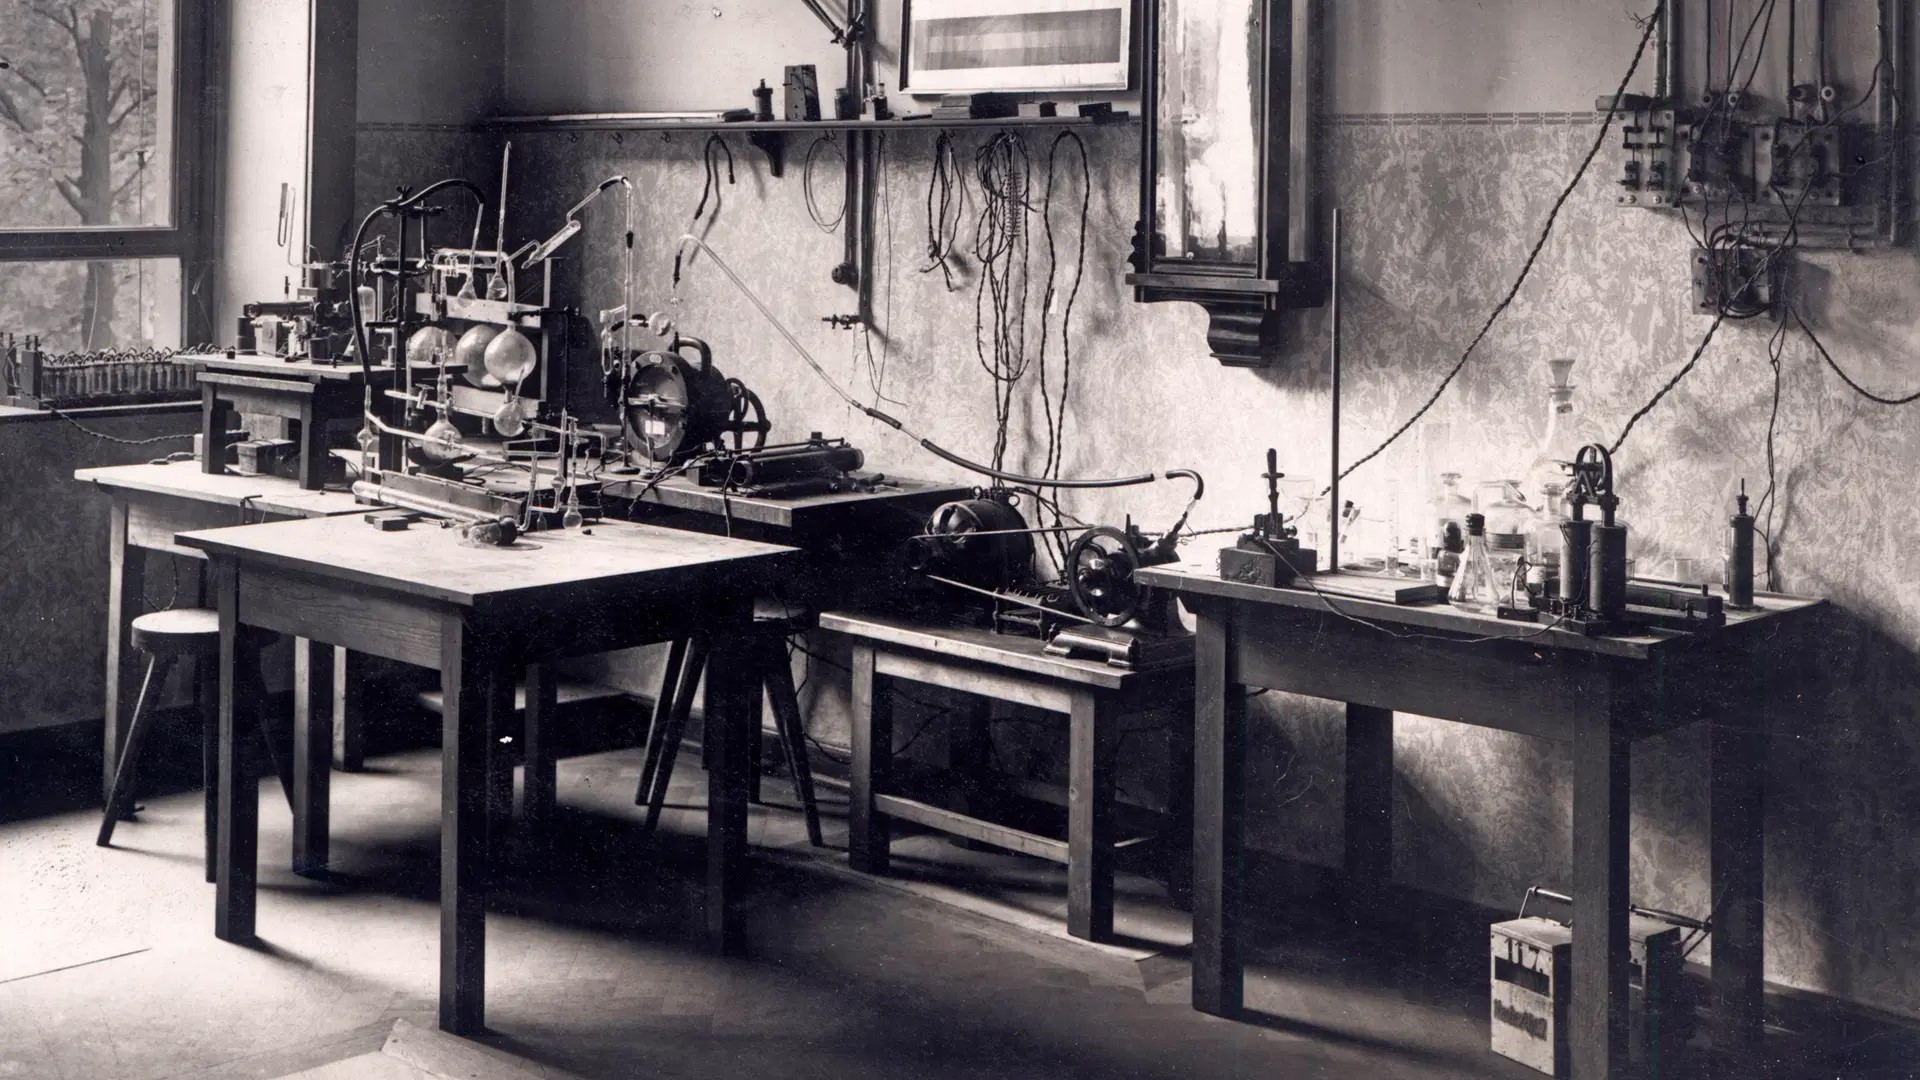
\includegraphics[scale = 0.2 ]{lab.jpg}
  \captionof{figure}{Röntgen's lab at the University of Würzburg (Credit : German Röntgen Museum)}
  \label{lab}
\end{center}

His lab in the University of Würzburg was kind of spartiate but he had enough means to conducts every experiments he wanted. This is a particularity of German's research organisation. Even universities of small town receive consequent subventions. This with the aim of promoting initiatives.

Röntgen, obviously because of it technical school background and a intrinsic curiousity, was an extremely fine experimenter. This is characteristic of its knowledge and work. After his discovery, he said \textit{I was not thinking, only searching}... Always, he had deep humility, often this was too much toward his talent.

In January 1896, Röntgen demonstrated his groundbreaking discovery to the German medical-
physical society. A compelling moment during this demonstration involved creating an X-ray
image of the hand of Albert von Kölliker, a prominent anatomist of that era (refer to Fig. 7.4).
This live demonstration immediately convinced Röntgen's colleagues of the practical significance
of his invention.
\newpage
\begin{center}
  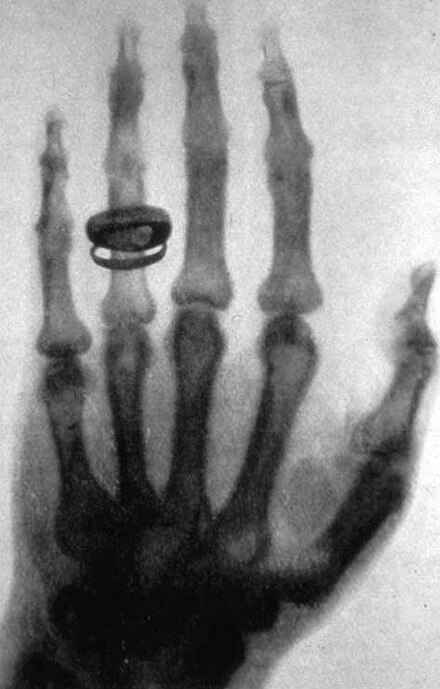
\includegraphics[scale= 0.3]{KollikerHand.jpg}
  \captionof{figure}{X-ray of Kölliker's hand, made by Röntgen on 23 Jan 1896 (Credit : German Röntgen Museum )}
  \label{KollikerHand}
\end{center}

While the appearance of these photographs was described as ghastly, the article emphasized their
significant scientific implications. The practical applications of this discovery were extensive,
including the ability for surgeons to use this new form of photography to precisely locate
embedded bullets in the human body or visualize fractures in bones before surgical procedures.
The method also held promise for addressing conditions such as caries and other bone diseases.
The Vienna Press assured its readers that this was a serious and genuine discovery by Professor
Röentgen, marking the birth of radiology.
Despite his reputation for being quiet and reserved, it is ironic that Röntgen's discoveries
garnered instant global attention. This can be attributed to another aspect of his character.
Röntgen's willingness to forgo patenting his findings allowed researchers worldwide to explore
and experiment with X-rays. He firmly believed that his "inventions and discoveries belong to the
world at large."

\chapter{The Discovery of X-Rays}
In this chapter we will reveal Röntgen's experimental setup and methodology, the moment of his discovery. Then we will show the first X-ray images, and the reaction of the public and scientific world after the discovery.

\section{Impact of Röntgen's X-Rays discovery}

In this section, we will reveal Röntgen's experimental setup and methodology, the
moment of his discovery. Then we will show the first X-ray images, and the reaction of
the public and scientific world after the discovery.

Wilhelm Röntgen's accidental discovery of X-rays in 1895 marked a seismic shift in the
realms of medicine and physics. The serendipitous moment, capturing the image of his fingers
on a cardboard screen, set the stage for an unprecedented revolution. Within months, X-rays
found applications in medicine, with studies initiated to explore vascular anatomy and the
gastrointestinal tract. The rapid dissemination of Röntgen's findings worldwide showcased the
extraordinary impact of this breakthrough. By 1896, over a thousand scientific papers on X-
rays had been published, with widespread implications for both medical and physical
sciences. Industrial advancements, such as Thomas Alva Edison's contributions, further
propelled the transformative wave. This discovery pushed other physicist to explore the X-ray
spectrum, with the discovery by Compton/Rayleigh of high/low energy waves. Röntgen's
recognition culminated in numerous honors, including the inaugural Nobel Prize for Physics
in 1901, underscoring the enduring influence of his revolutionary discovery.
\newpage
For example, Henri Poincaré, a French great physician, congratulated Röntgen in a letter \footfullcite{PoincaréToRontgen} for his experience and discovery. It reveals a real enthusiasm. Please have a look.

\begin{center}
  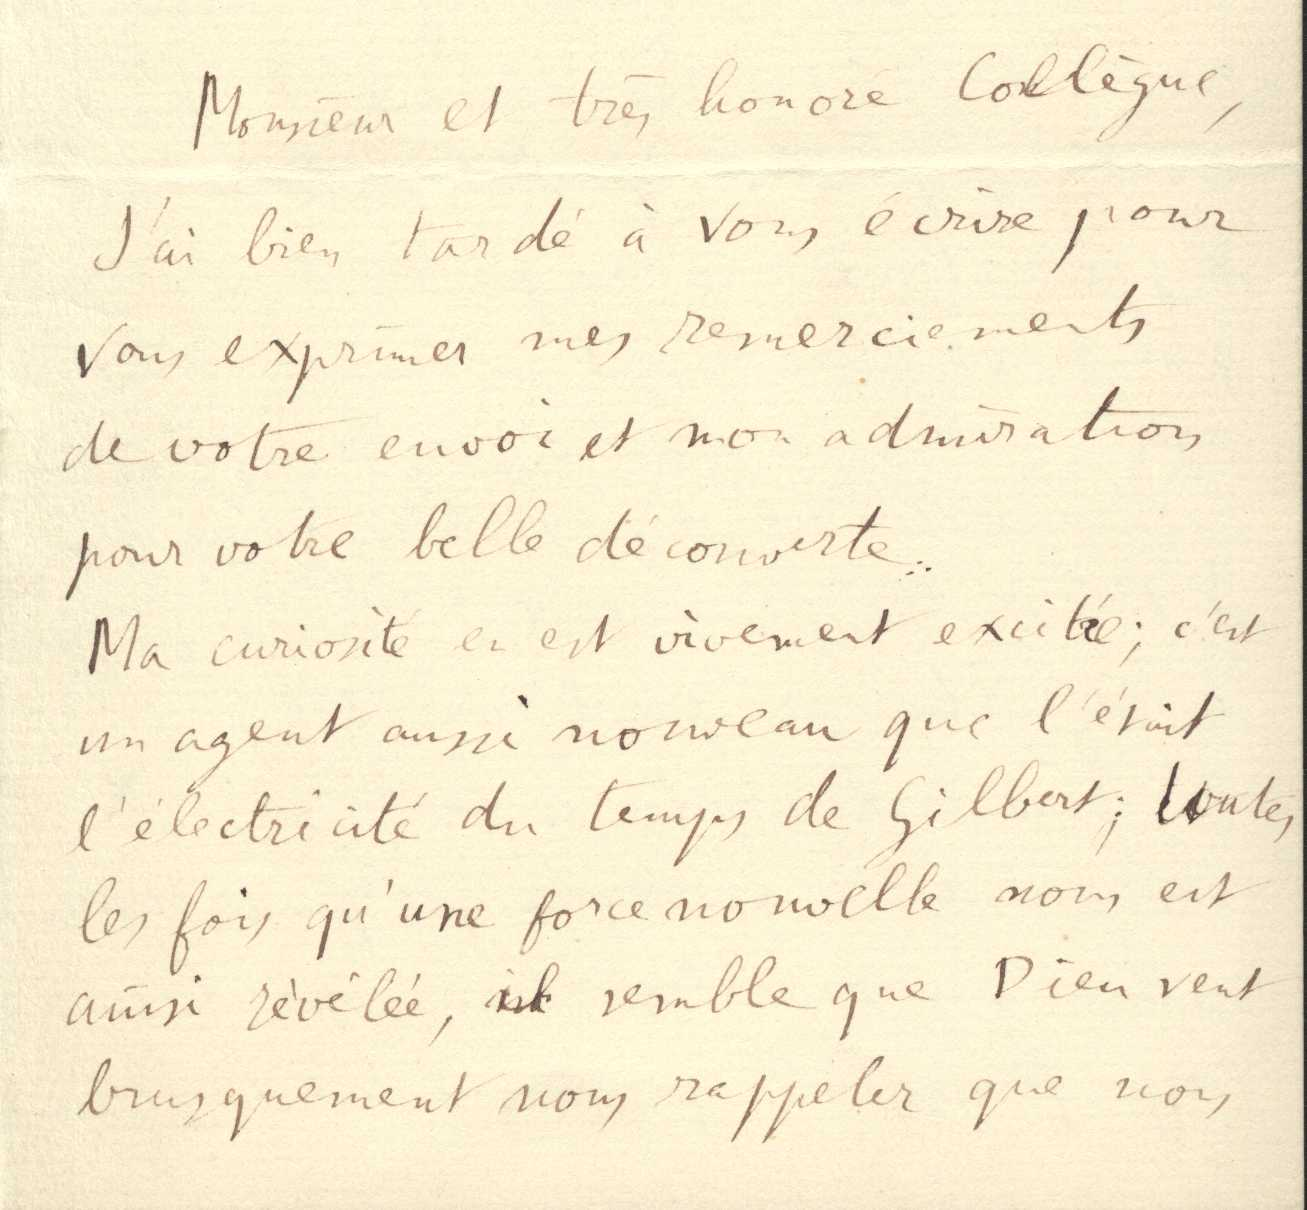
\includegraphics[scale = 0.8]{letter1.jpg}
  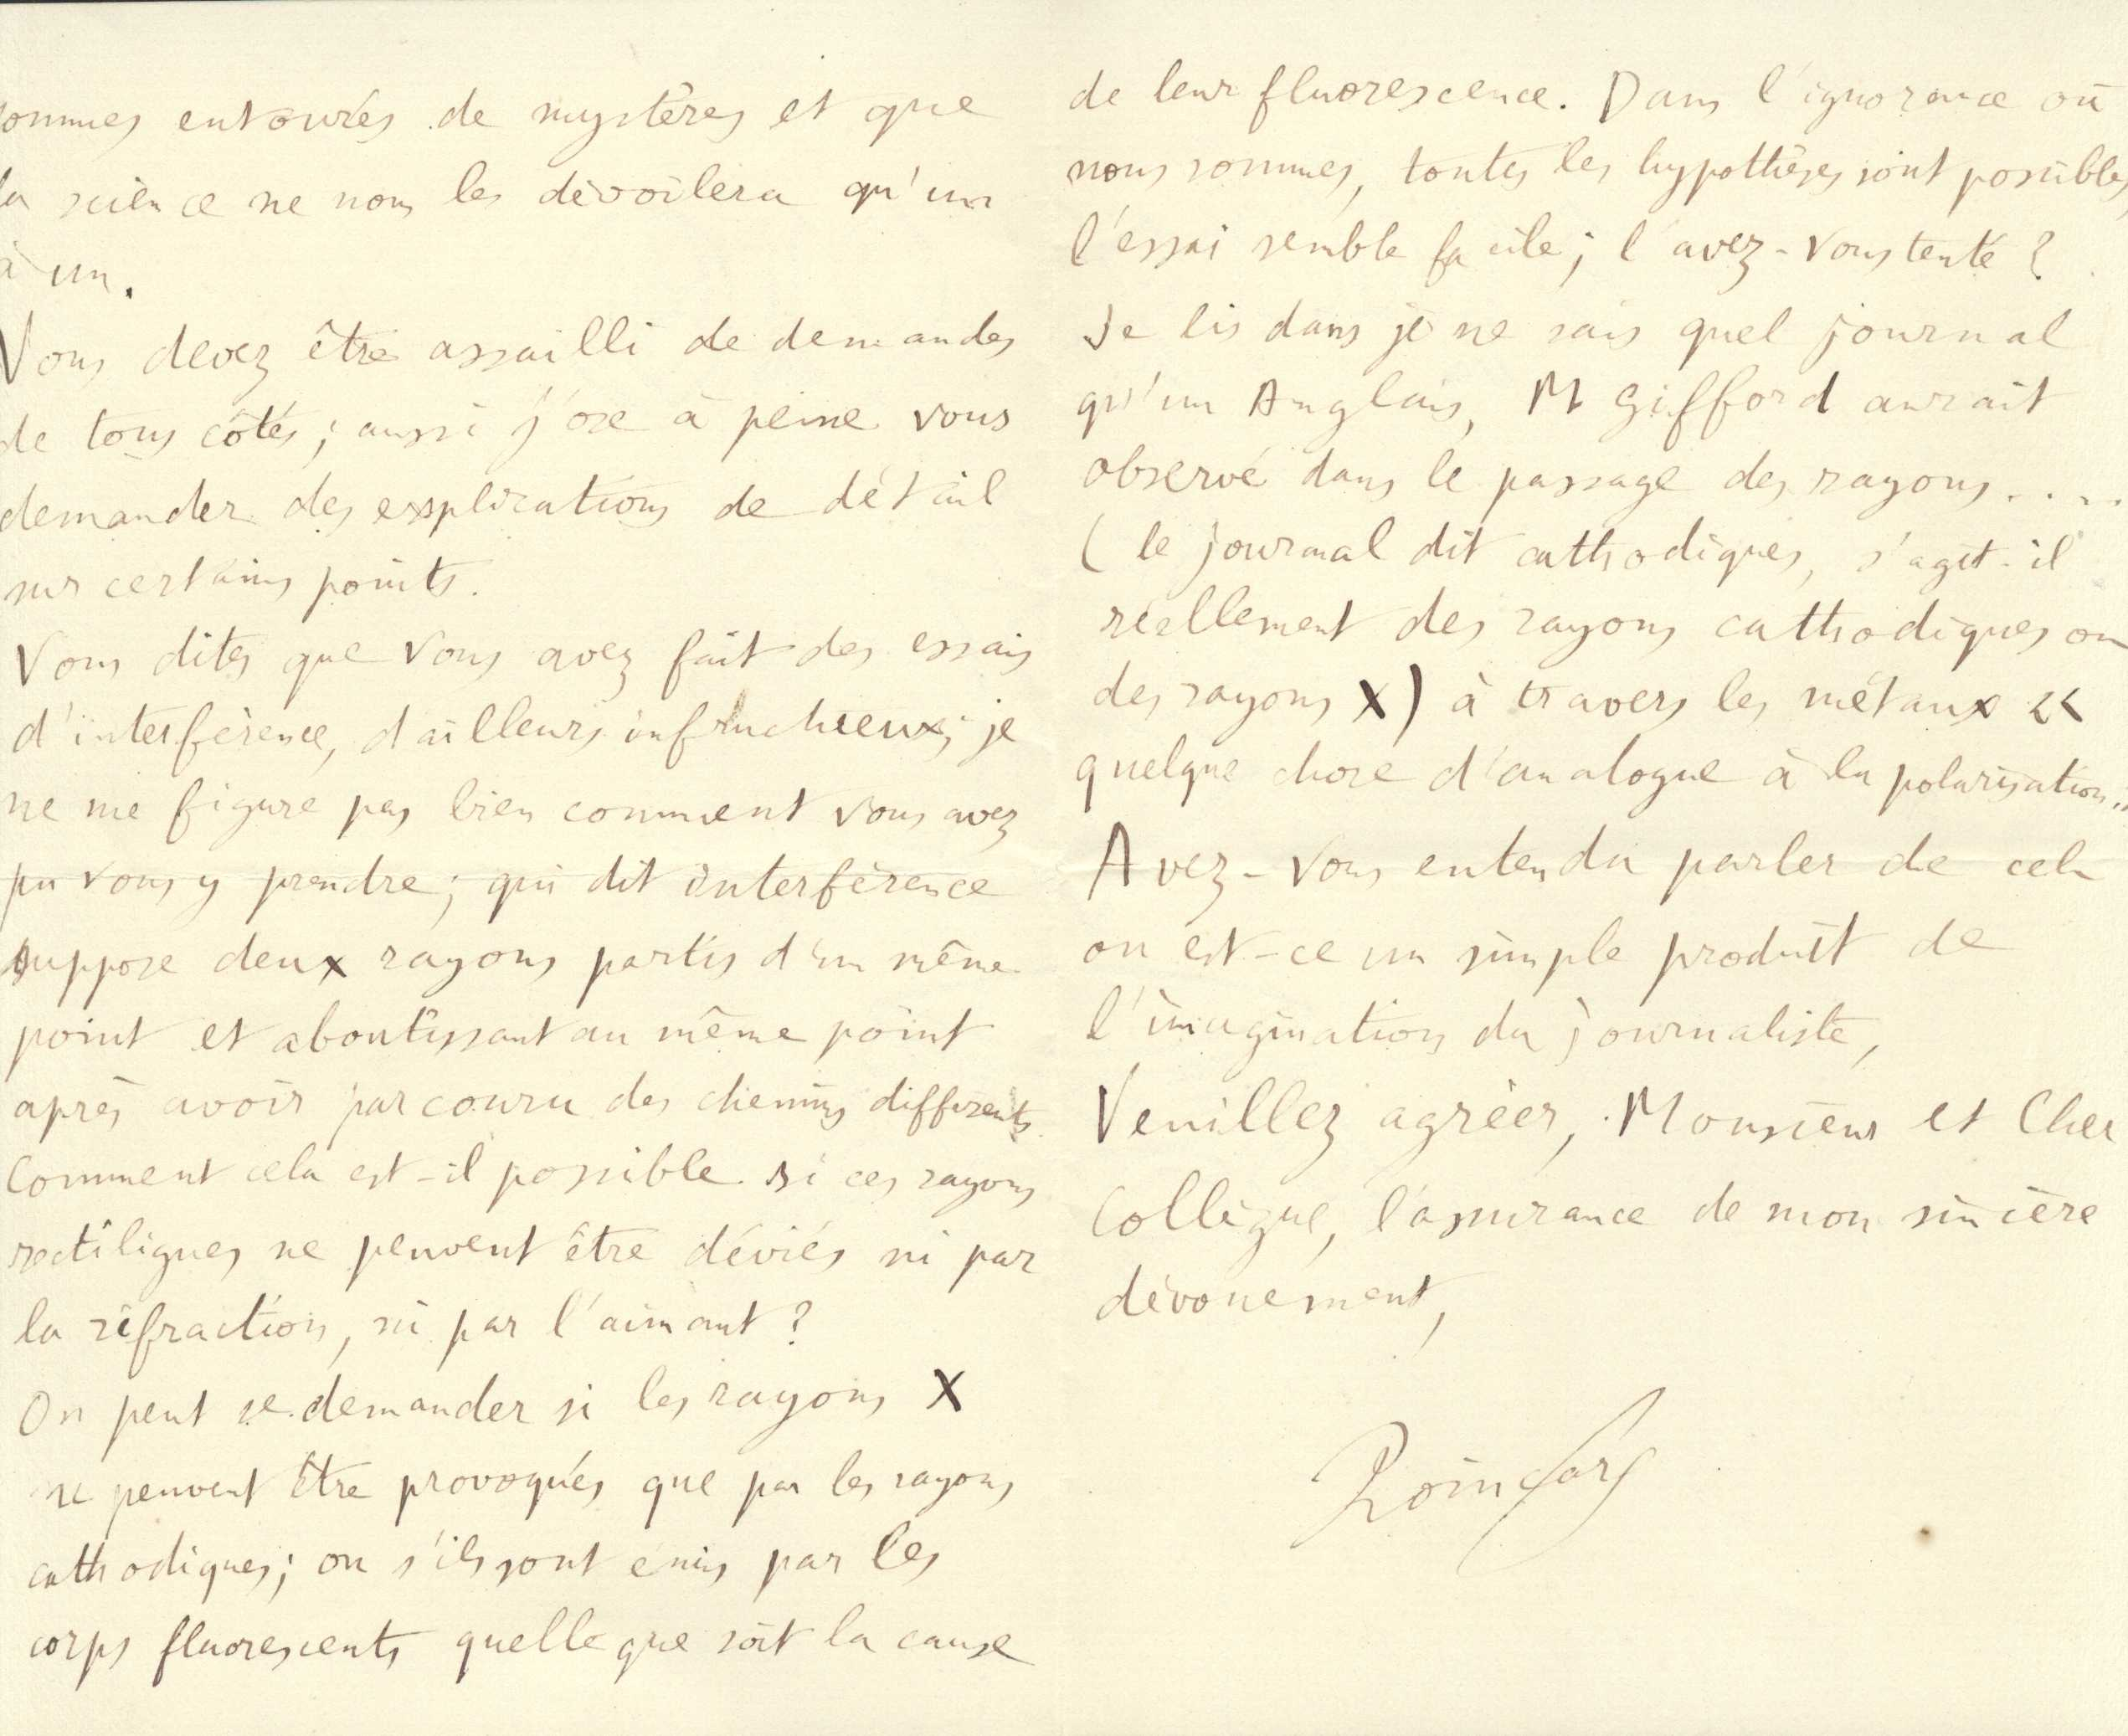
\includegraphics[scale = 0.6]{letter2.jpg}
  \captionof{figure}{Letter from H. Poincaré to W. C. Röntgen }
\end{center}

\newpage
Here is a transcript and translation of some sentences.
\begin{multicols}{2}

  \textit{
  J'ai bien tardé à vous écrire pour vous exprimer mes remerciements de votre envoi et mon admiration pour votre belle découverte.(...) }
  
  \textit{Ma curiosité en est vivement excitée; c'est un agent aussi nouveau que l'était l'électricité du temps de Gilbert.(...)}
  
  \textit{Vous devez être assailli de demandes de tous côtés; aussi j'ose à peine vous demander des explications de détail sur certains points.(...)
  On peut se demander si les rayons X ne peuvent être provoqués que par les rayons cathodiques; ou s'ils sont émis par les corps fluorescents quelle que soit la cause de leur fluorescence.}
  

  \columnbreak 
  \textit{
  I have been quite delayed in writing to you to express my gratitude for your shipment and my admiration for your wonderful discovery. (...)}
  
\textit{
  My curiosity is greatly aroused by it; it is an agent as novel as electricity was in Gilbert's time. (...)}
  
\textit{
  You must be inundated with requests from all sides; therefore, I hardly dare to ask you for detailed explanations on certain points. (...)
  One may wonder whether X-rays can only be provoked by cathode rays, or if they are emitted by fluorescent bodies regardless of the cause of their fluorescence. (...)}

\end{multicols}

This piece of history from 1896, announces well how revolutionary this discovery is. Poincaré makes a comparison with discovery of electricity.



\section{Explanation and phenomenons behind Rongtens discovery}
\subsection{Crookes's Tube}
The main tool at the disosal of Röntgen was a cathode-rays tube. Known today as \textit{ Crooke's Tube} from the name of the invento
r a british physician.

\begin{center}
  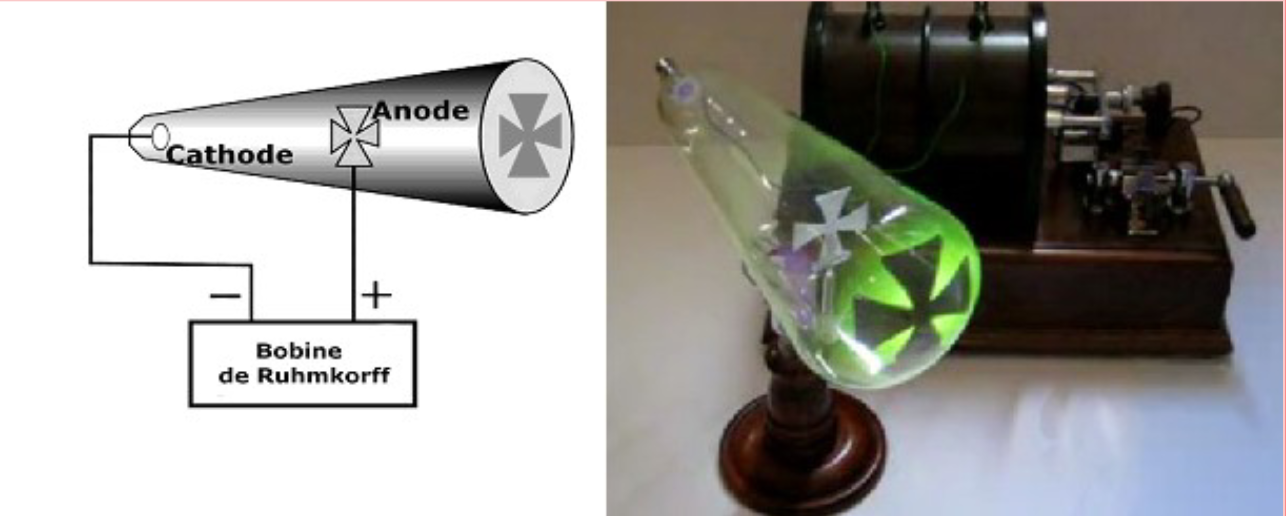
\includegraphics[scale = 0.7]{tubeCrookes.png}
  \captionof{figure}{A Crooke's Tube and its schematic}
  \label{tubeCrookes}
\end{center}

This tube is the firt means of observation for X-rays. It is a vacuum-sealed glass
tube housing a cathode and a solid metal anode. In a classical X-ray tube, there's a part called the
cathode with a heated filament. When this filament gets really hot, it releases electrons. These
electrons are then pushed or accelerated by the tube's electric power (voltage) from the cathode
(negative side) to the anode (positive side). When these speedy electrons hit the anode, they slow
down and change direction because of the anode's electric field. This slowing down process
creates electromagnetic waves, and specifically, it produces X-rays. So, in simpler terms, the X-
ray tube works by heating up a filament to release electrons, accelerating these electrons with
electric power, and then letting them hit a metal target, which produces X-rays in the process.

The anode is angled at a specific degree to guide the X-rays in the intended direction. Normally,
each electron undergoes multiple slowing down or deflection actions, leading to the production of
several photons. Nevertheless, there's a possibility that an electron loses all its speed and energy
in a single step. In such instances, only one photon is generated, encompassing the entire energy
of the electron.

It is important to note that cathode-rays observed originally in Crookes tube are rays of electrons and therefore may be deviated by an electric or magnetic field. According to Röntgen experiments this is not the case, X-rays are longitudinal and can not be deviated by electric or magnetic field. We demonstrate later that is because X-rays has no charge.
\begin{center}
  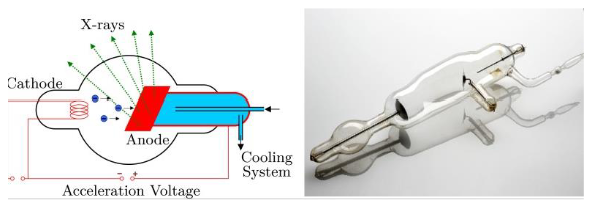
\includegraphics[scale = 1.5 ]{modernTube.png}
  \captionof{figure}{A more modern Crooke's Tube with its schematic (Credit : Science Museum, London)}
  \label{modernTube}
\end{center}


The modern vacuum X-ray tube, depicted in the images, operates through the acceleration of electrons
from the cathode to the anode, ultimately leading to the generation of X-ray photons. In the
schematic on the left, the acceleration of electrons is illustrated as they travel from the cathode to
the anode within the vacuum tube. This process results in the production of X-ray photons. The
image on the right displays a historical vacuum X-ray tube, providing a tangible representation of
the technology. This visual insight into the apparatus underscores the significance of these tubes
in the historical development of X-ray imaging.


\begin{center}
  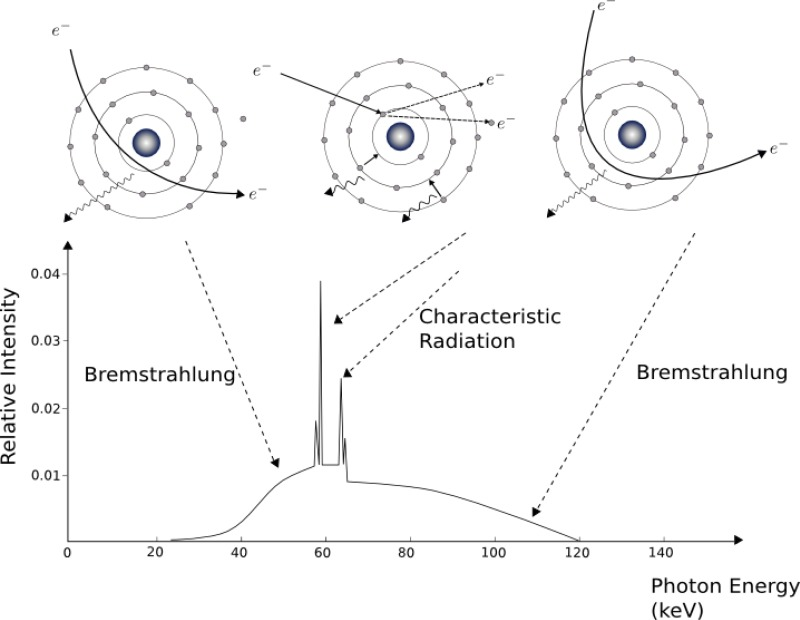
\includegraphics[scale = 0.5]{xraytungsten.jpg}
  \captionof{figure}{X-ray spectrum of a tungsten tube. (Credit : NCBI Bookshelf)}
  \label{xraytungsten}
\end{center}

The X-ray spectrum produced by a tungsten tube exhibits characteristic radiation peaks, with the
continuous portion of the spectrum representing Bremsstrahlung.

This report \footfullcite{IntroductoryGuide} explained the peculiar nature of invisible light rays, revealing that wood and other
organic materials were transparent to these rays, while metals and bones, whether human or
animal, were opaque. This meant that these rays could be absorbed by bones or metals enclosed
in a wooden or woolen covering, enabling the photographing of bones or metals within such
materials. The article noted that human flesh, being organic, behaved similarly, allowing the
photography of bones without the accompanying flesh appearing on the plate. Vienna already had
photographs demonstrating this, showcasing human hand bones along with rings worn on the
fingers.

\newpage

\subsection{Ruhmkorff Coil}
Crookes tube is nothing without a high voltage pulse generator called \textit{Ruhmkorff's Coil}. It is necessary to provide high electric discharge for the radiation.The following figure explains the operation.
\begin{multicols}{2}
  \begin{center}
    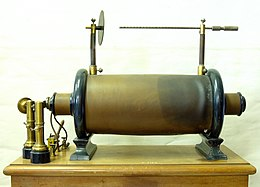
\includegraphics[scale=0.6]{ruhmkorff.jpg}
    \captionof{figure}{Original Ruhmkorff Coil }
  \end{center}
  \columnbreak
  \begin{center}
    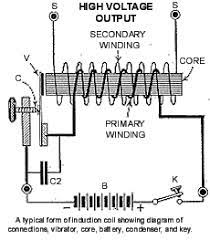
\includegraphics[scale=0.5]{schemRuhm.jpeg}
    \captionof{figure}{Diagram of a Ruhmkorff Coil }
  \end{center}
\end{multicols}


Röntgen used generally a current of 20 A to generate adequated sparks.


\subsection{The Lambert-Beer's Law}

To understand the apparition of more or less dark spot. The \textit{Lambert-Beer 's Law} is necessary.

The Beer-Lambert law asserts that the absorbance of a solution is directly proportional to its
concentration. Here is the relation.

\begin{equation}
  I = I_0 \cdot e^{- \mu x}
\end{equation}

Here I is the intensity output, \(I_0\) is the intensity input, \(\mu\) is the linear attenuation coefficient.
It is important to note that this formulation works inside liquid solution.
This formula is derived from a first order homogenous differential equation of the radiation
intensity.

\begin{equation}
  \frac{dI}{dx} = - \mu I
\end{equation}

Therefore, we may show that biological matter such as bone or soft tissue have different absorption properties. It follows X-Rays densities for human body.

\subsection{The 5 X-ray densities}
The contrast observed in an overall medical image is contingent on variations in both the density
and thickness of anatomical structures within the body. The extent of contrast between two
adjacent structures within the image is directly proportional to the disparities in either the density
or thickness of those structures. Descriptively, five distinct densities can aid in discerning the
characteristics of abnormalities. Notably, unexpected changes in the density of a recognized
anatomical structure, whether an increase or decrease, can provide valuable insights into the
tissue composition of the abnormality, aiding in its identification and characterization.

\begin{center}
  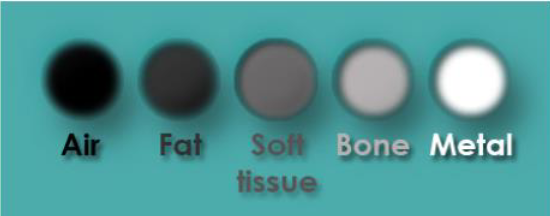
\includegraphics[scale = 1.2]{xraydensity.png}
  \captionof{figure}{5 different colours according to type of matter\footfullcite{masterclass}}
  \label{5densities}
\end{center}

The classification of X-ray densities encompasses five distinct categories. Low-density
substances, like air, are visualized as black on the final radiograph, while highly dense materials
such as metal or contrast agents appear as white. Bodily tissues exhibit a range of grey tones,
dictated by both their density and thickness. This grayscale spectrum allows for nuanced
differentiation among various anatomical structures, facilitating a comprehensive and detailed
interpretation of X-ray images in medical diagnostics


\section{Radiography's Early Applications and Pioners}
Here, we will dive thought on how Röntgen's discovery led to the development of radiography. We will also discuss about the pioneers in radiography who followed Röntgen We will finalize by talking about the early applications of radiography in medicine and industry.
\subsection{Wilhelm Conrad Röntgen: Pioneer of Radiology}
Wilhelm Conrad Röntgen, the founder of radiology, made a transformative discovery in 1895 by
accident. While experimenting with cathode-ray tubes and glass, he uncovered invisible rays
capable of passing through most substances, naming them "X-rays." Röntgen's groundbreaking
work led to the publication of "On a New Kind of Rays" on December 28, 1895. His findings spread
rapidly, and by February 1896, clinical applications of X-rays had begun. Röntgen's remarkable
contributions earned him the first Nobel Prize in physics in 1901, establishing the foundation for
modern radiology.
\subsection{Study of Crystal atomic structures}

Röntgen at his time thought that diffraction was not possbible with X-rays. This was a big question weeks after his discovery, but he did not continue researches on the subject. 
However during his life other scientists found a way to differentiate authentic diamonds with fakes one using radiology. Fake diamonds, made at the time with very dense type of glass, observed a lot more absorption than real ones that were almost transparent. The reason why is true diamonds are crystal with well organised atomic structure letting radiations go through. Whereas fakes one had disorganised structure more opaque.

This observation was the premisces of using X-rays diffraction to precisely determined the atomic structure of crystal.
Nowadays\footfullcite{Diffraction}, the technique is very powerful and used in chemistry. Calculations based on diffraction spot resolve the atomic structure or monocrystal.

\begin{multicols}{2}
  \begin{center}
    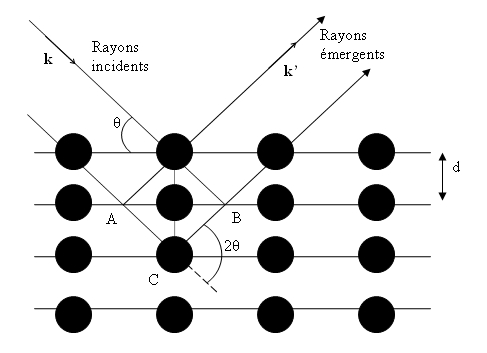
\includegraphics[scale=0.5]{diffraction.jpg}
    \captionof{figure}{Reflection of X-rays by a family of lattice planes spaced at a distance d }
  \end{center}
  \columnbreak
  \begin{center}
    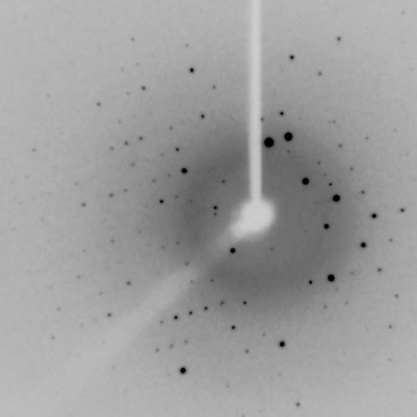
\includegraphics[scale=0.4]{crystal.jpg}
    \captionof{figure}{Image obtained during the exposure of a single crystal to an X-ray beam.}
  \end{center}
\end{multicols}

\subsection{Evolution of Radiology Technology}
The history of radiology technology evolved from early glass photographic plates to contemporary
digital imaging and archiving technologies like PACS/MIMPS. In contrast to traditional X-ray
films, which directly utilize X-rays to alter the chemical properties of the film material, modern
detection systems follow a different approach. They initially convert X-rays into light and
subsequently transform this light into electrons for the imaging process. The progression continued
with significant leaps, including George Eastman's introduction of film in 1918. Advances persisted
with the advent of ultrasound technology post-World War II, followed by the introduction of
computed axial tomography (CAT scan) and magnetic resonance imaging (MRI) in the 1970s.

\begin{center}
  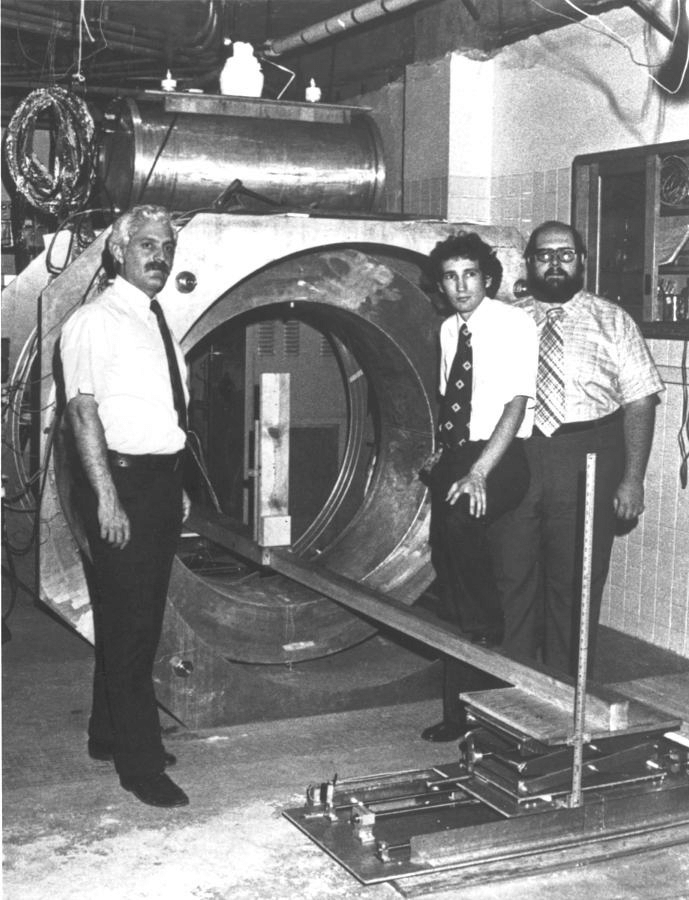
\includegraphics[scale =0.3]{firstMRI.png}
  \captionof{figure}{R. Damadian, L. Minkoff, M. Goldsmith and the "Indomitable," the world's first MRI scanner which they developed (Credit : BBC)}
  \label{firstMRI}
\end{center}

\subsection{Timeline of Advances in Radiology}
The timeline of advances in radiology marks significant milestones in medical imaging
technology. In 1895, Wilhelm Röntgen's discovery of X-rays revolutionized the field, laying the
foundation for future developments. Fast forward to 1972, when Godfrey Hounsfield introduced
the first CT scanner, a groundbreaking innovation that provided detailed cross-sectional images
of the body. In 1977, Raymond Damadian achieved another milestone with the completion of the
first MRI, offering a non-invasive method for imaging soft tissues. The turn of the millennium
brought recognition to the PET-CT scanner, named the medical invention of the year in 2000,
highlighting the ongoing strides in enhancing diagnostic capabilities and patient care through
radiological advancements

\subsection{Transformative Journey}
From glass plates to cutting-edge digital modalities, radiology has revolutionized patient care.
Technological advances have given rise to tailored software solutions like PACS, RIS/PACS
integrations, teleradiology, and Imaging EMRs, setting the gold standard for 21st-century medicine
and healthcare administration. The journey, highlighted by groundbreaking discoveries and
innovations, continues to shape the future of radiology and healthcare delivery.

\chapter{Advances  in Radiographic Technology}
\section{Evolution of Radiography Equipment and Techniques}
Here, we will talk about the evolution of radiographic equipment and techniques. 
 
\begin{center}
  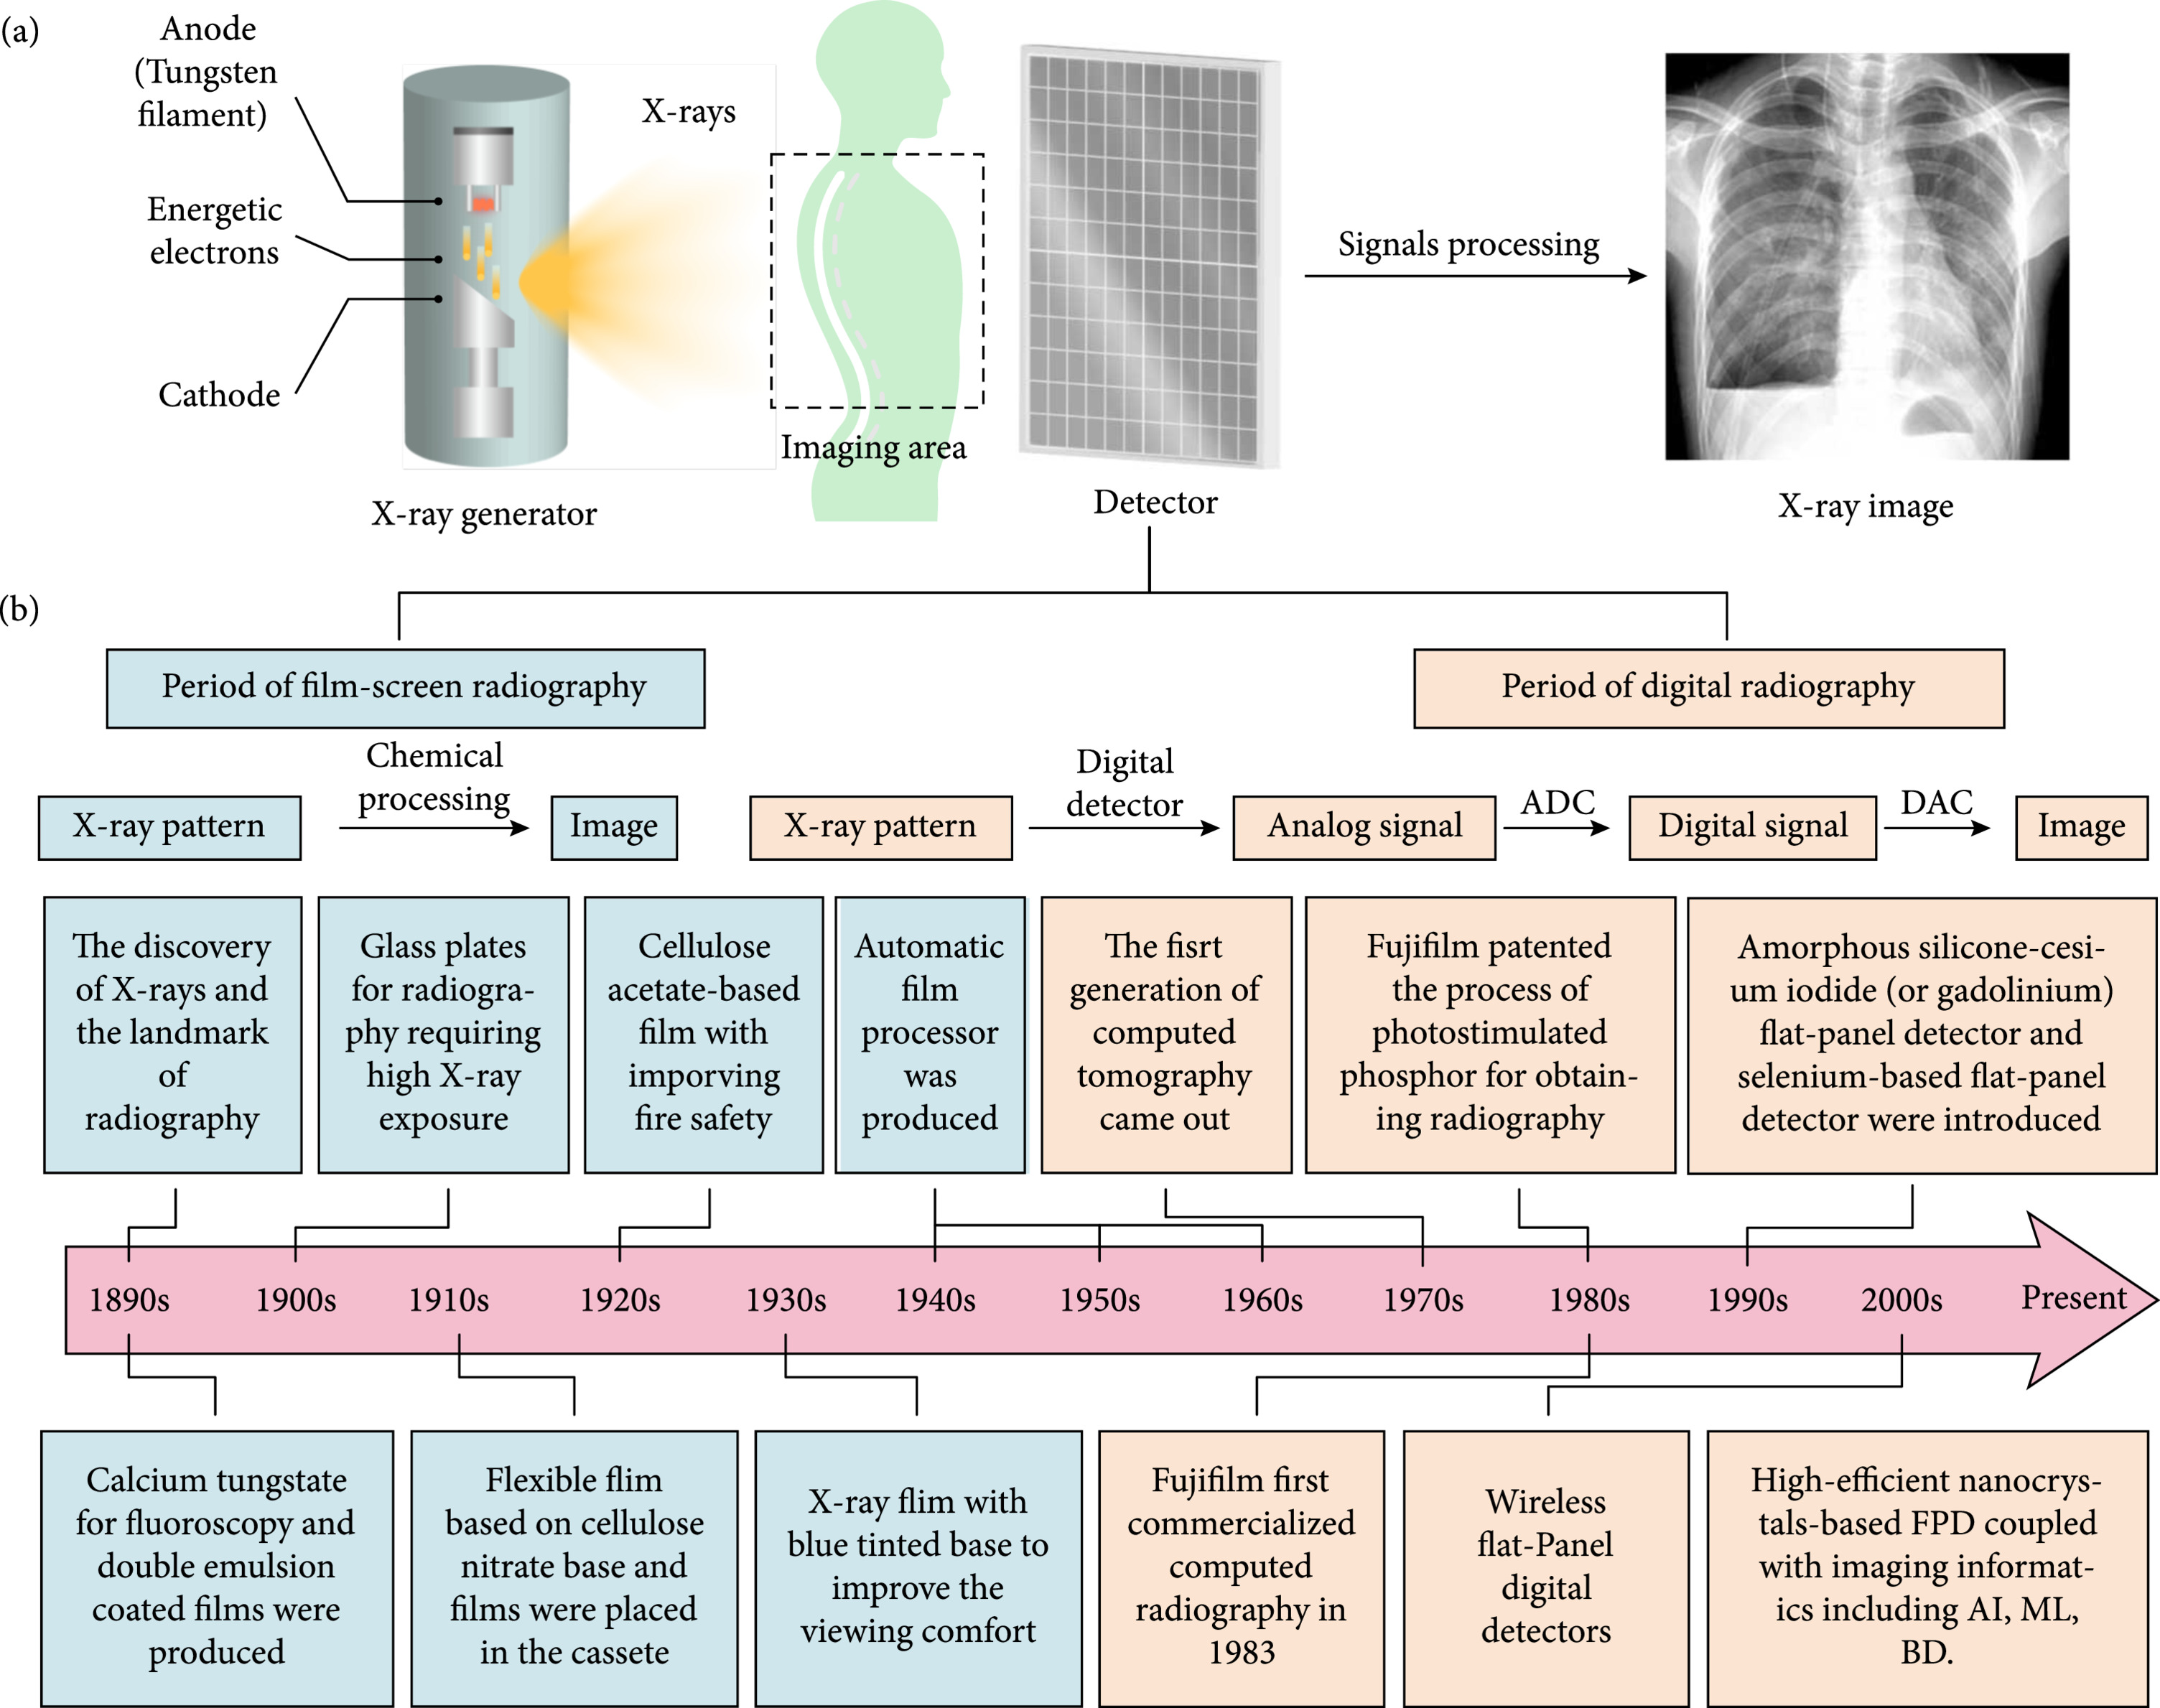
\includegraphics[scale = 0.5]{chrono.jpg}
  \captionof{figure}{(a) Schematic illustration of an X-ray imaging system. (b) The development of X-ray radiography with the evolution of X-ray detectors}
  \label{chrono}
\end{center}

\section{	Technological Breakthroughs in Radiography}

We will follow up by discussing technological breakthroughs in radiography. 

In this era, patients underwent notably invasive tests, and awareness of the hazards
associated with radiation exposure was on the rise. The 1970s marked a transformative
period in radiology, often referred to as the "golden decade," as the introduction of the CT
scanner ushered in a new era of possibilities and groundbreaking discoveries. The
advancements made during this time laid the foundation for further innovations in the
subsequent decades, particularly in the 1980s and 1990s.

To better understand the progress in the field, it is helpful to categorize each decade into
distinct areas of focus. These subdivisions encompass radiology, radiography,
radiotherapy, radiobiology, medical physics, and diagnostic imaging. By examining
developments within these specialized domains, one can gain a comprehensive overview
of the dynamic evolution of medical imaging and radiation-related disciplines over the
years.

\section{Radiography During World War I and II}
We will extend this chapter by talking about the impact of World War I and World War II on radiography. 

Soon after Wilhelm Roentgen's discovery of X-rays in late 1895, their application in medical
operations swiftly emerged. Recognizing their utility, military surgeons embraced X-rays for
identifying broken bones, bullets, and shrapnel in wounded soldiers. This newfound technology
played a crucial role in diagnosing injuries during various conflicts, including the Greco-Turkish
War, the Russo-Japanese War, and the Balkan Wars over the next few years. To support field
hospitals, mobile units were developed, ensuring that X-rays could be readily available wherever
surgery was performed, underscoring their vital role in advancing medical practices on the
battlefield.

In 1914, Marie Skłodowska Curie, already renowned for her groundbreaking work in
radioactivity, including the discovery of radium and polonium, found a practical application for
20
her expertise when World War I erupted in Europe. Recognizing the potential of X-rays in aiding
the treatment of wounded soldiers, Curie saw an opportunity to make a significant impact on
battlefield medicine.

\begin{center}
  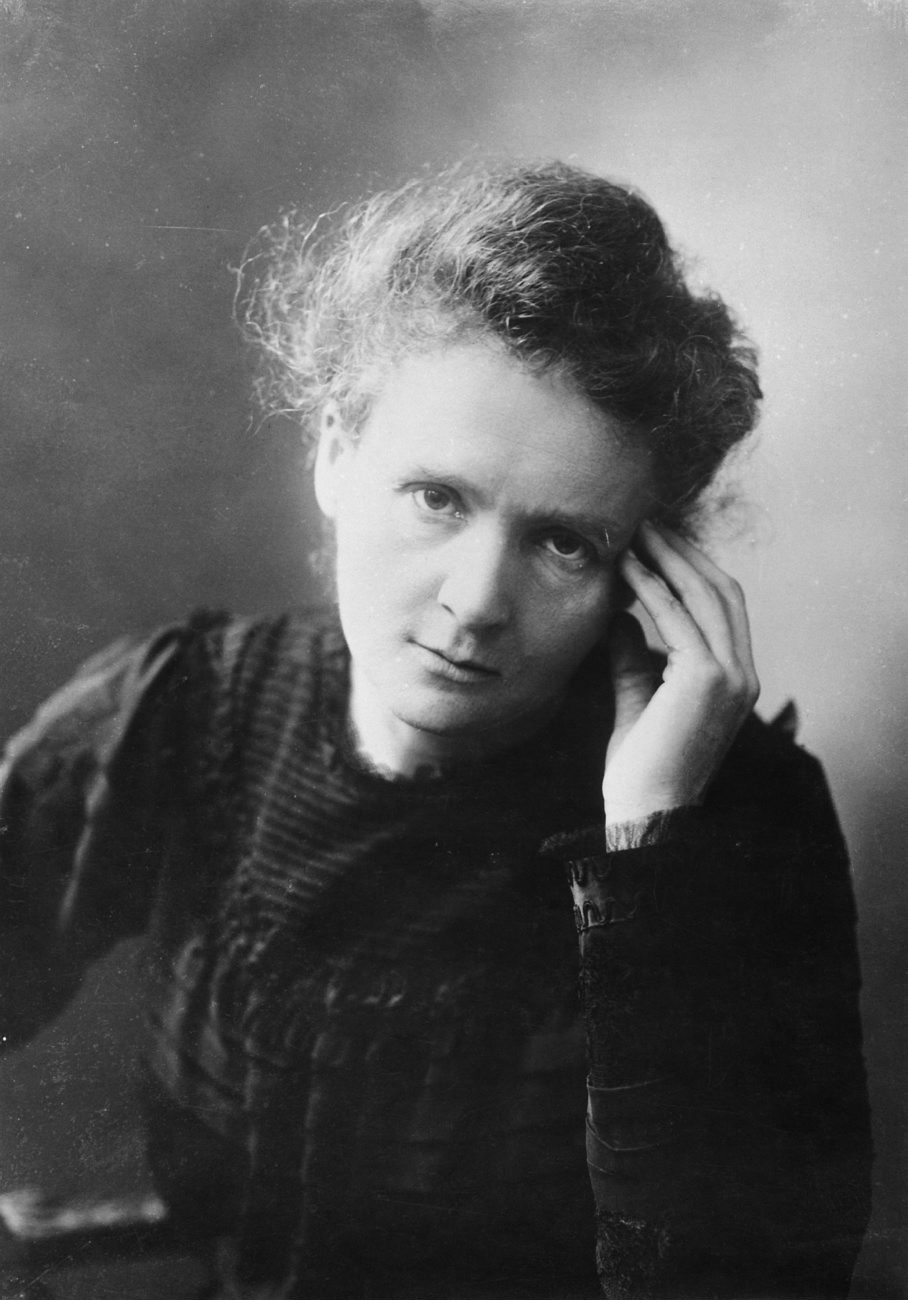
\includegraphics[scale = 0.2]{curie.jpg}
  \captionof{figure}{Portrait of Marie Curie. First female to win the Nobel prize (Credit : Flickr/Okänd)}
  \label{curie}
\end{center}

Understanding that X-rays could assist in locating and extracting bullets, shrapnel, and
identifying broken bones within the bodies of injured soldiers, Curie took action to bring this
technology closer to the front lines. Despite many hospitals in France having X-ray equipment,
the machines were often situated far from the immediate battlefield.


\begin{center}
  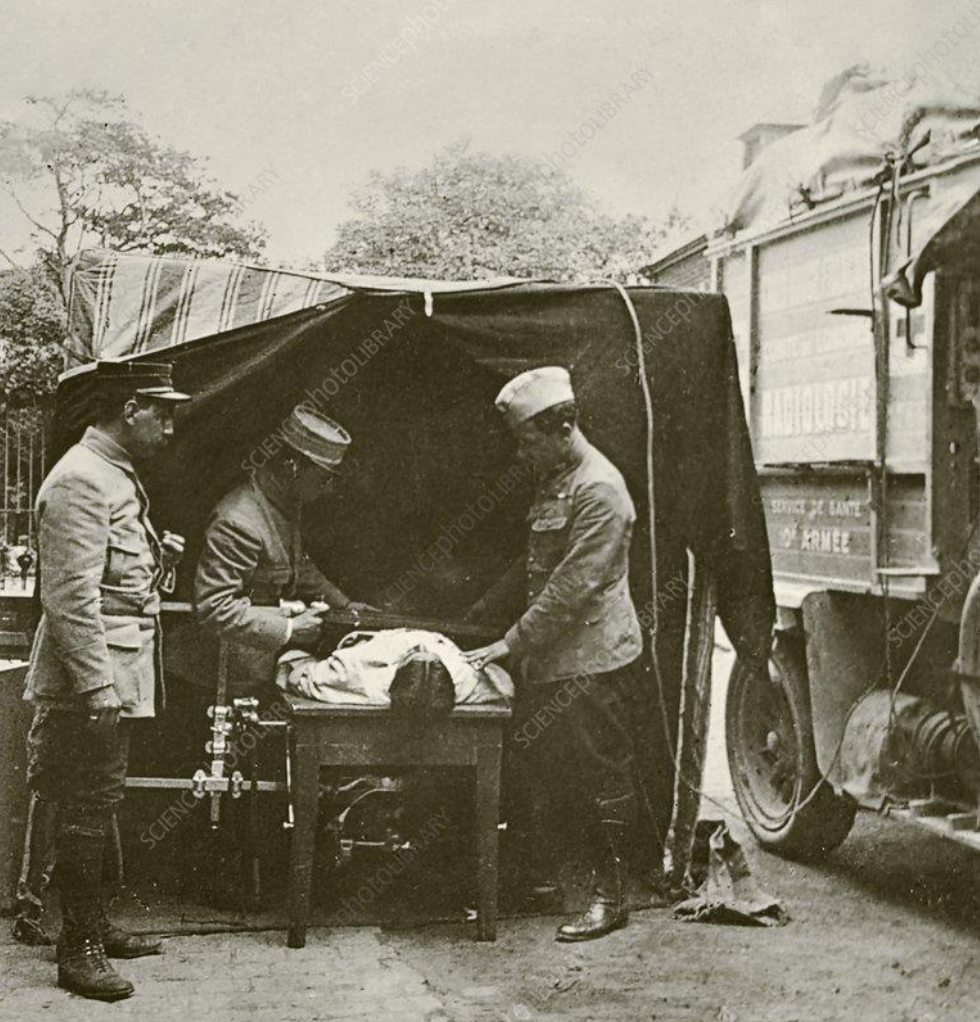
\includegraphics[scale =0.5]{mobileUnit.png}
  \captionof{figure}{A mobile X-Ray Unit during WW1 } 
  \label{mobileUnit}
\end{center}

To bridge this gap, Curie and her daughter organized a fleet of vehicles equipped with X-ray
machines. Over the first two years of the war, they established 200 radiological units in more
permanent posts, strategically placing them closer to the areas where medical attention was
urgently needed. This initiative, spearheaded by Curie, played a vital role in improving the
efficiency of medical care on the battlefield, showcasing the innovative application of scientific
knowledge to address urgent wartime challenges.

The advances in technology, particularly the widespread use of X-rays during the First World
War, held profound significance on two fronts. Firstly, they directly contributed to saving lives
by enhancing the medical response to injuries, especially those caused by gunshot wounds and
shrapnel. The ability to swiftly and accurately identify foreign objects within the body facilitated
more effective surgical interventions, thereby increasing the chances of survival for wounded
soldiers.

Secondly, these technological advancements played a crucial role in preventing illness by
addressing the persistent threat of infection. Infection, a major cause of fatalities throughout the
war, posed a significant challenge to medical care. By aiding in the precise detection and removal
of foreign objects, X-rays contributed to minimizing the risk of infection and its subsequent
spread. Consequently, the integration of cutting-edge technology not only improved immediate
patient outcomes but also played a pivotal role in mitigating the secondary health risks associated
with wartime injuries.

To ensure timely medical intervention on the front lines during wartime, the development of
portable X-ray equipment became crucial. Recognizing the significance of proximity in
enhancing the chances of saving lives, military x-ray units were established to deploy this
technology efficiently. Casualties typically undergo multiple stages of care, emphasizing the
importance of having X-ray capabilities as close to the front line as possible. The responsive
solution was the creation of mobile X-ray units, equipped with portable machines that could
swiftly and effectively be set up in field hospitals and forward medical stations. This strategic
deployment aimed to minimize the time between injury and diagnosis, facilitating prompt and
targeted medical responses in critical situations.

\begin{center}
  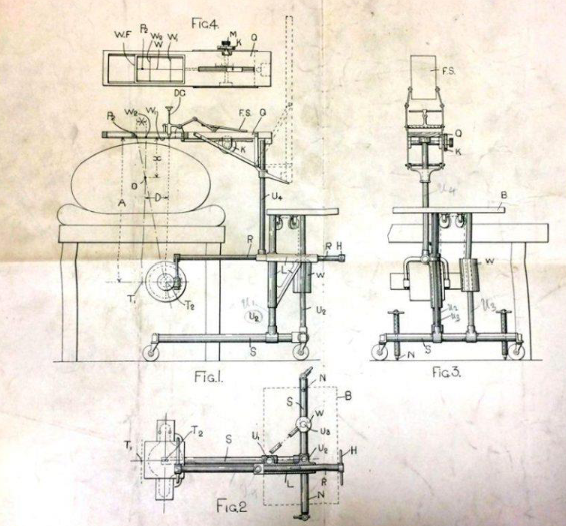
\includegraphics[scale = 1]{drawing.png}
  \captionof{figure}{Assembling schematic of a mobile Unit for X-Rays}
  \label{drawing}
\end{center}

\chapter{Modern Applications of Radiography}
\section{Contemporary Uses and Challenges in Radiography}
We will emphasize here the contemporary uses of radiography in medicine, industry, and other fields, along with the benefits and challenges of modern radiographic technology.

Radiological technology, once in a disruptive phase, is now transitioning into a sustaining phase,
presenting a spectrum of challenges and opportunities that shape the future of medical imaging.
Two critical challenges in medical imaging are the pursuit of precise, noninvasive tissue
characterization and the enhancement of micro resolution for early lesion detection. Despite its
current share of only 5 \% of total healthcare expenditure, concerns about the affordability of
imaging technology arise due to its increasing costs amid rapid utilization. The perception of
radiologists as 'invisible' figures, secluded in dark cubicles, poses a challenge in the era of
digitalized medicine and virtual visits. The evolution towards in vitro diagnostics (genomics,
proteomics) is a challenge but offers potential solutions for earlier disease diagnosis,
revolutionizing radiological screening policies

On the flip side, numerous opportunities await the field. Quantitative imaging, with its emphasis
on precision and evidence-based medicine, holds the potential for growth. Improved networking
and communication facilitated by Picture Archiving and Communication Systems (PACS) and
Radiological Information Systems (RIS) offer active sharing of databases, contributing to 'value-
based radiology.' Interventional radiology stands out as a significant opportunity, minimizing
invasiveness and lowering costs through advanced techniques and semi-automated guidance
software. The integration of over 50 billion connected devices, including medical devices, in the
coming years presents opportunities for telemonitoring, emergency notification systems, and
portable laboratory testing, revolutionizing the diagnostic approach.

Examining technological advancements in X-ray imaging since 1895 reveals ongoing efforts to
address challenges. The search for advanced X-ray energy converting materials continues to
achieve low-dose, high-resolution, large-area, and flexible X-ray detectors. Technical hurdles, such
as scintillation decay, synthesis processes, and optical crosstalk, persist but must be overcome for
practical radiography. Metasurface technology, combining high-efficiency X-ray converting
layers, emerges as a promising strategy to enhance X-ray sensitivity. On going developments aim
to create large-area and flexible X-ray imaging detectors, opening possibilities for applications in
dental X-ray inspections, imaging irregular objects, and portable X-ray testing.

In conclusion, while radiological technology faces challenges in evolution, the fusion of
innovation, adaptability, and advancements offers a promising future for medical imaging, where
precision, accessibility, and patient-centric approaches take center stage

\chapter{Ethical and Safety Considerations in Radiography}

\section{Ethical and Safety issues in Radiography}
We will talk about ethical and safety issues related to radiographic procedures\\

The historical development of regulations for radiation protection. Initially, individuals sought
protection through professional guidelines, with the German Roentgen Society providing
guidelines in 1913. George Pfahler in the U.S. urged the creation of guidelines, emphasizing the
mastery of radiology principles and legal protection for radiologists. In 1927, the National Bureau
of Standards initiated a voluntary inspection program for radiation equipment. The International
Commission on Radiological Protection (ICRP) and the U.S. Advisory Committee on X-Ray and
Radium Protection played pivotal roles in formulating guidelines. Concepts like "tolerance dose"
and "maximum permissible dose" were established, with ongoing revisions based on health risks
rather than arbitrary limits. The Nuclear Regulatory Commission (NRC) emerged in 1974 to
separate conflicting objectives and continue regulatory functions, ensuring a balance between
fostering nuclear technologies and protecting public health.

\section{Development of Safety Protocols and Regulations}

Medical imaging's centrality to patient care, akin to labs or pathology, has spurred concerns about
radiation safety dating back to the field's inception. Over the last decade, several states, following
California's lead, have mandated enhanced radiation dose management, presenting a considerable
operational challenge for healthcare providers. Dose Management Systems (DMS) have emerged
as vital support in navigating these regulations. The imperatives for dose management excellence
encompass data aggregation and processing, ensuring compliance with regulations and best
practices, leveraging visualizations for insights, interoperability with existing IT infrastructure,
and scalability. Modern DMS, exemplified by Siemens Healthineers' Teamplay Dose, address
these imperatives, providing easy access to dose data, supporting quality assurance, and offering
advantages such as reduced infrastructure costs and continuous feature releases, thus contributing
to the systematic monitoring of patient radiation dose with enhanced efficiency and efficacy

The development of safety protocols and regulations in the context of radiation exposure is
crucial, considering the intricate nature of its effects on living organisms and the environment.
Nuclear power reactors, while containing the majority of radioactivity, still emit a small
percentage as gas or liquid effluent, contributing to global background radiation. Despite efforts
to minimize exposure, cancer treatments involve doses significantly larger than environmental
radiation, underscoring the need for stringent safety measures. Radioactive releases from nuclear
bomb explosions or accidents can contaminate the atmosphere and water over long distances,
emphasizing the importance of regulatory frameworks to mitigate such risks. The impact of
radiation on cells, including interference with division and damage to chromosomes and genes,
necessitates careful consideration in safety protocols. Gene mutations escalate with radiation
dose, emphasizing the significance of dose accumulation rate. Furthermore, early-life radiation
exposure has been linked to reduced longevity in laboratory animals due to the induction of
benign and malignant growths. While some substances offer protection against radiation, their
toxicity limits practical application in humans. Activities involving radiation exposure are
rigorously assessed for risks in medicine, science, and industry, with a concerted effort to avoid
unnecessary exposure. The benefits of radiation in medical procedures are weighed against risks,
particularly in population-wide screenings. Additionally, non-ionizing radiation, such as Hertzian
waves and infrared rays, poses heating effects, necessitating safety considerations in various
applications, including diathermy, microwave ovens, and occupational exposure limits. The
ongoing development of safety protocols and regulations remains essential to navigate the
complex landscape of radiation and ensure the well-being of both humans and the environment.

\subsection{The invere square law}

\textit{The inverse square law states that for a point source of waves that is capable of radiating omnidirectionally and with no obstructions in the vicinity, the intensity I decreases with the square of the distance, d, from the source. \footfullcite{telco}}

Understanding the 'inverse square law' is instrumental in minimizing radiation exposure.
Essentially, this principle asserts that by reducing the distance from the radiation source by half,
the dose to a specific area becomes quadrupled. In simpler terms, maintaining a distance from a
radiation source is an effective means of decreasing the radiation dose to personnel. This
becomes especially crucial in interventional radiology scenarios where radiologists or
radiographers often operate in close proximity to the X-ray beam.

The intensity of the X-ray beam exhibits an inverse square relationship with the distance from the
source (X). Specifically, doubling the distance from the radiation source, from 'd' to '2d,' results
in a reduction of the dose to the radiologist or radiographer to one-fourth of the original amount.
This underscores the importance of maintaining a safe distance from the radiation source to
mitigate exposure risks effectively.

\chapter{Wilhem Conrad Röntgen's Legacy}
\section{Importance of Radiation Dose Management}

he evolution of X-ray-based radiology examinations since their discovery in 1895 and the
subsequent increase in patient radiation dose exposure, particularly with the adoption of
multidetector computed tomography (MDCT). The public's heightened interest in radiation
exposure, fueled in part by events like the Fukushima nuclear disaster, has led to concerns about
medical radiation exposure.

The Korean National Evidence-Based Healthcare Collaborating Agent (NECA) published a
report \footfullcite{NECA} in 2011, emphasizing that radiation exposure from the Fukushima disaster in Korea was
minimal and below harmful levels. It highlights the need for public education to dispel vague
fears of medical radiation exposure, emphasizing the benefits outweighing the disadvantages.

The International Commission on Radiological Protection (ICRP) emphasizes the importance of
using radiation exposure to benefit patients while optimizing protection. The principle of "As
Low As Reasonably Achievable" (ALARA) guides radiology studies to minimize radiation dose
without compromising patient care.

The text underscores the increasing importance of monitoring, optimizing, and decreasing patient
medical radiation exposure globally. Efforts to educate the public and healthcare professionals on
proper radiation knowledge are deemed insufficient, and the focus is shifting toward systemic
and organized approaches for managing radiation dose.

The subsequent section delves into radiation dose units, explaining concepts such as exposure,
absorbed dose, equivalent dose, and effective dose. The importance of understanding these units
in the context of medical radiation management is highlighted. The text concludes with a table
summarizing the relationships between different radiation dose units.




\section{Lasting Impac and Legacy Röntgen}

Wilhelm Conrad Röntgen's discovery of X-rays in the late 19th century had a profound and
lasting impact on science, medicine, and technology. This breakthrough earned him the first
Nobel Prize in Physics in 1901 and inspired generations of scientists. Röntgen's legacy is
commemorated through the "Röntgen," a unit of measurement for X-ray and gamma-ray
intensity, as well as various medical institutions and awards bearing his name.

\begin{center}
  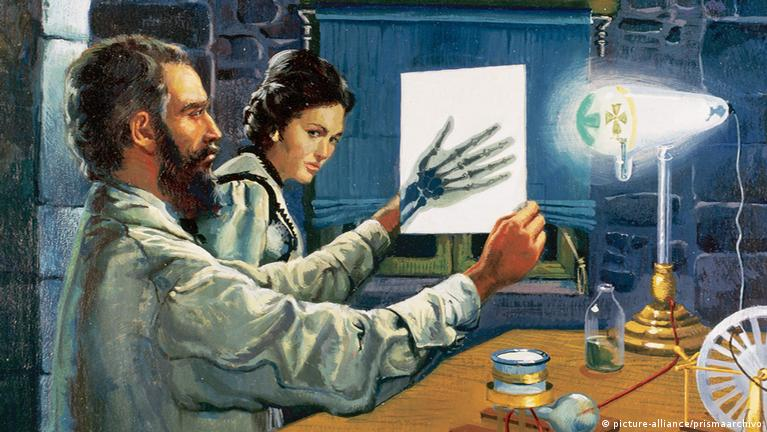
\includegraphics[scale = 0.6]{wr.jpg}
  \captionof{figure}{Artistic view of X-ray discovery, W.C. Röntgen and his wife Anna Bertha Ludwig. (Credit : picture-alliance/primaarchivo)}
\end{center}


His meticulous approach to experimentation and emphasis on documentation set a standard for
scientific research. Beyond his immediate discoveries, Röntgen's work ignited scientific curiosity
globally, leading to the development of other imaging techniques like MRI and ultrasound.
Despite his groundbreaking achievements, Röntgen remained humble and selflessly refused to
patent his discovery, advocating for free accessibility for the benefit of humanity.

While Röntgen's X-ray discovery revolutionized medical imaging, it also prompted concerns
about potential risks. Over time, stringent safety measures and guidelines were established to
ensure responsible use, minimizing harm to both patients and healthcare professionals. Röntgen's
contributions continue to shape the field of medicine and exemplify the spirit of inquiry that
propels scientific advancements


\section{Recognition and Honors for Röntgen}
In this chapter we will talk about the lasting impact of Röntgen's work on X-rays and radiography. Then we will see the recognition and honours he received, and how his legacy continues to influence the field.

Wilhelm Conrad Röntgen, the pioneering physicist, received widespread recognition and honors
for his revolutionary discovery of X-rays. In 1901, he was awarded the first inaugural Nobel
Prize in Physics, an esteemed acknowledgment that solidified his position as a trailblazer in the
scientific community. The establishment of the Nobel Prizes was not a direct response to
Röntgen's discovery but rather a broader initiative by Alfred Nobel to recognize and reward
outstanding achievements across various fields that contribute to the betterment of humanity.
Röntgen's legacy is further immortalized through the naming of the unit of measurement for X-
ray and gamma-ray intensity, known as the "Röntgen" or "Roentgen." Numerous medical
institutions, research centers, and awards globally bear his name, underscoring the profound
impact of his contributions. The German Physical Society established the Röntgen Memorial
Lecture, providing a platform for distinguished scientists to honor his legacy and present their
research. 

Beyond accolades, Röntgen's meticulous approach to experimentation and his
humanitarian gesture of refusing to patent his discovery have set enduring standards in scientific
research. His influence extends globally, inspiring generations of scientists and shaping the field
of medical imaging. Röntgen's recognition encompasses not only his scientific achievements but
also his lasting impact on the spirit of inquiry and the ethical principles that guide scientific
advancements

\begin{center}
  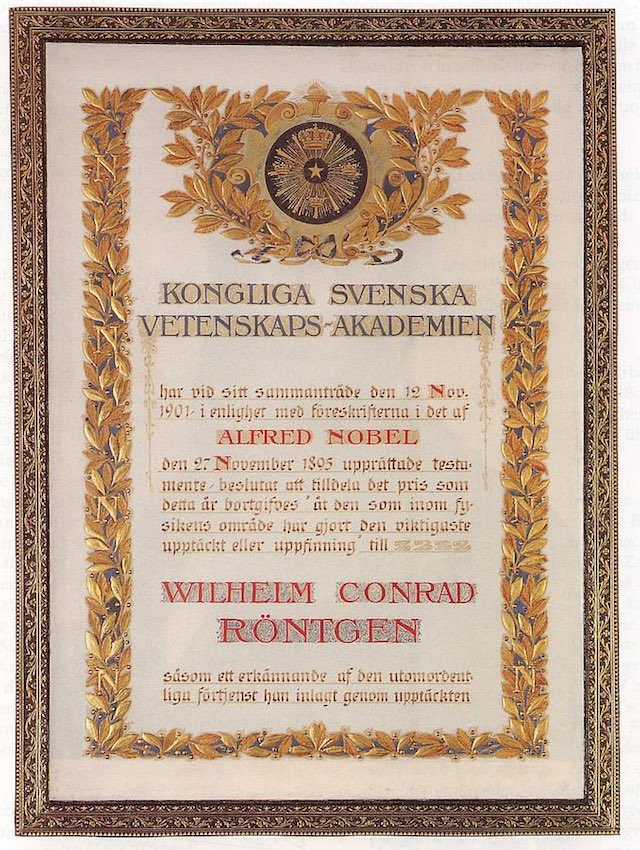
\includegraphics[scale = 0.25]{nobelpreis.jpg}
  \captionof{figure}{Röntgen's Physics Nobel Prize, the first in History. (Credit : Röntgen Memorial)}
\end{center}

\chapter{Future Trends in Radiography}
\section{Emerging Technologies and AI in Radiography}

Here we will discuss and argue about the potential advancements and innovations in radiography. The emerging technologies and applications in the field, and the role and influence that of artificial intelligence could have inradiography.

The integration of artificial intelligence (AI) into radiography is a growing trend, and the
future role of radiographers is expected to involve working with AI-based tools. The provided
text emphasizes the importance of robust validation for new AI tools using unseen data,
advocating for more prospective interdisciplinary research and comprehensive approvals. The
involvement of service users, including practitioners, patients, and their caregivers, is deemed
essential in the design and implementation of AI tools. Additionally, the text stresses the need
for clearer accountability and medicolegal frameworks in cases of erroneous results from AI-
powered software and hardware. It calls for clearer career pathways, role extension provisions,
and education in the field, recognizing the central role AI will play in healthcare. The paragraph
highlights the expectation that AI applications in medical imaging will evolve to be more
accurate, cost-effective, and widely accessible, potentially improving patient-centered care and
precision medicine. The convergence of efficiency, increased patient throughput, and a focus
on patient well-being is seen as a goal for the future of radiographic practice with AI

\chapter{Conclusion}

In summary, Wilhelm Röntgen's breakthrough in discovering X-rays has left an enduring and
transformative mark on the realms of radiography and medical imaging. His innovative
contributions provided the groundwork for the evolution of sophisticated imaging
methodologies, fundamentally altering the landscape of medical practice. The continuous
progress in radiography technology further refines X-ray imaging, enabling more precise
diagnoses and elevating standards in patient care. Despite these advancements, a crucial
emphasis is placed on maintaining awareness of radiation safety and optimizing dosage to
address potential risks linked to ionizing radiation.

In 1894, Röentgen had stated: “The scientist must considerthe possibility, which usually amounts
to a certainty, that his work will be superseded by oth-ers within a relatively short time, that his
methods will be improved upon and that the newresults will be more accurate and the memoryof his
life and work will gradually disappear.” Considerable advancements have occurred since
Röentgen's groundbreaking discovery in 1896. Nevertheless, the memory and reputation of this
selfless and gifted scientist are bound to endure and be esteemed.


\printbibheading

\printbibliography[type=book,heading=subbibliography,title={Books}]
\printbibliography[type=article, heading=subbibliography, title={Articles}]
\printbibliography[type=online,heading=subbibliography, title={Online Resources}]
\printbibliography[type=misc, heading=subbibliography, title={Other Documents}]
\listoffigures
\end{document} 
